\documentclass[tikz]{standalone}
\usepackage{amsmath}
\definecolor{bg}{HTML}{171D2B}
\definecolor{aksen}{HTML}{F7B538}
\definecolor{teks}{HTML}{FFFFFF}
\definecolor{biru}{HTML}{7DD3FC}
\definecolor{hijau}{HTML}{6EE7B7}
\color{teks}
\begin{document}
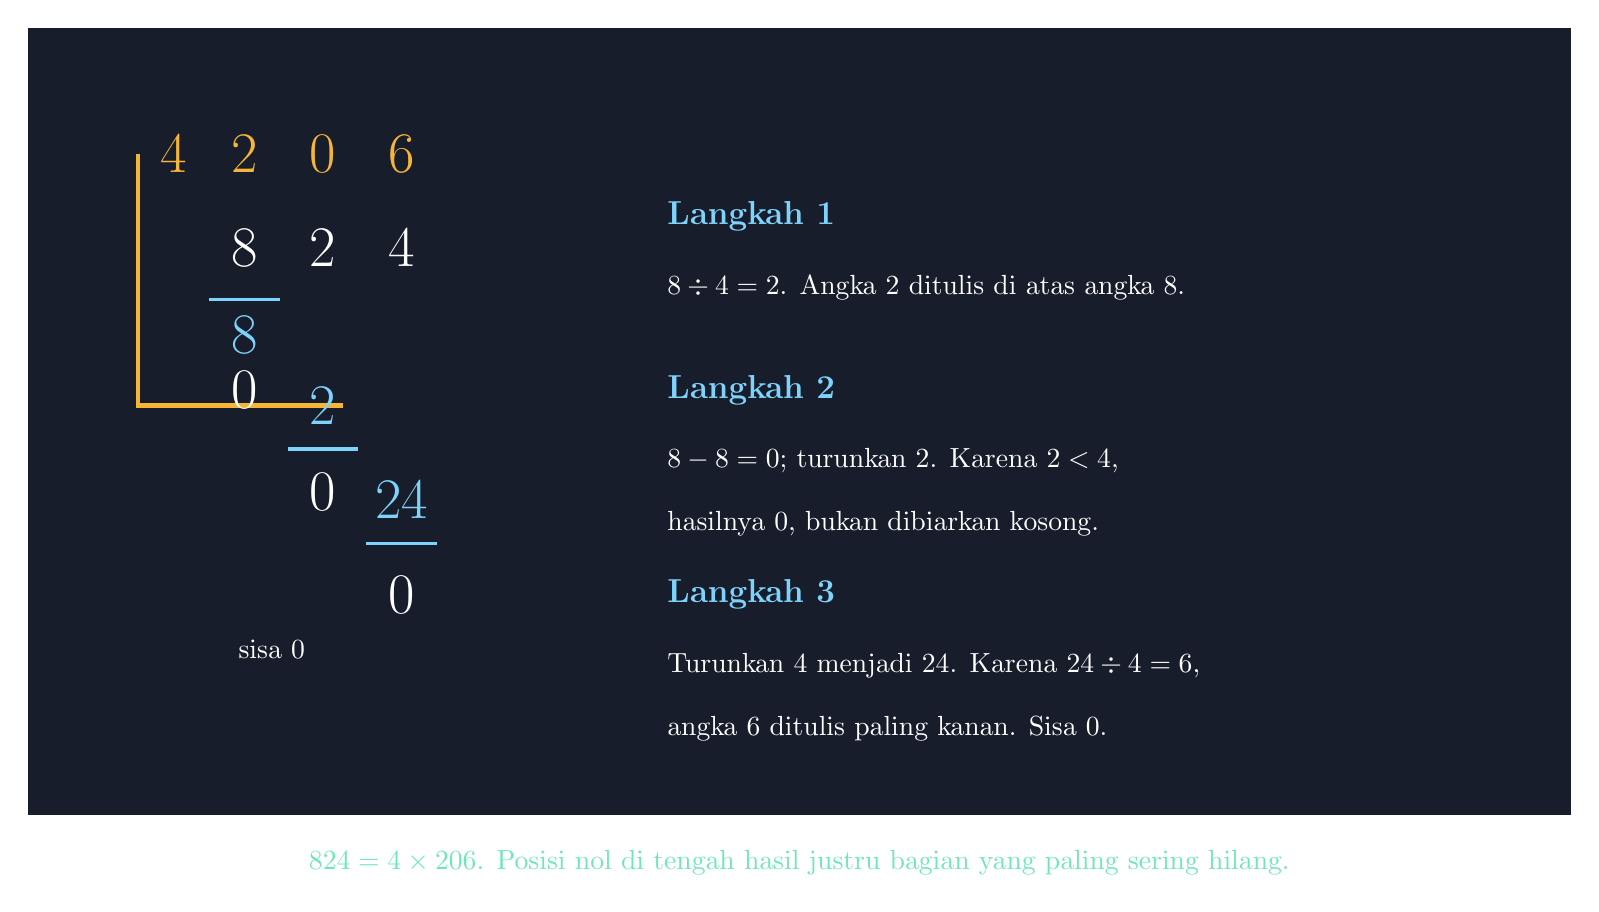
\begin{tikzpicture}[scale=1]
  \fill[bg] (-0.8,-1.0) rectangle (18.8,9.0);

  % ===== Panel kiri: porogapit 824 : 4 = 206 =====
  \begin{scope}[shift={(0.6,2.2)}]
    % tanda pembagian
    \draw[aksen, line width=1.6pt] (0,5.2) -- (0,2.0) -- (2.6,2.0);
    \node[aksen, font=\huge] at (0.45,5.2) {4};
    % hasil di atas (aksen)
    \node[aksen, font=\huge] at (1.35,5.2) {2};
    \node[aksen, font=\huge] at (2.35,5.2) {0};
    \node[aksen, font=\huge] at (3.35,5.2) {6};
    % 824
    \node[teks, font=\huge] at (1.35,4.0) {8};
    \node[teks, font=\huge] at (2.35,4.0) {2};
    \node[teks, font=\huge] at (3.35,4.0) {4};
    % langkah 1: 8-8
    \node[biru, font=\huge] at (1.35,2.9) {8};
    \draw[biru, line width=1.2pt] (0.9,3.35) -- (1.8,3.35);
    \node[teks, font=\huge] at (1.35,2.2) {0};
    % langkah 2: turun 2 (tetap), kurang 2-2
    \node[biru, font=\huge] at (2.35,2.0) {2};
    \draw[biru, line width=1.2pt] (1.9,1.45) -- (2.8,1.45);
    \node[teks, font=\huge] at (2.35,0.9) {0};
    % langkah 3: turun 4 jadi 24, 24-24
    \node[biru, font=\huge] at (3.35,0.8) {24};
    \draw[biru, line width=1.2pt] (2.9,0.25) -- (3.8,0.25);
    \node[teks, font=\huge] at (3.35,-0.4) {0};
    \node[teks, font=\normalsize] at (1.7,-1.1) {sisa 0};
  \end{scope}

  % ===== Panel kanan: tiga langkah =====
  \begin{scope}[shift={(7.2,6.6)}]
    \node[biru, font=\large\bfseries, anchor=west] at (0,0) {Langkah 1};
    \node[teks, font=\normalsize, anchor=west] at (0,-0.9) {$8 \div 4 = 2$. Angka 2 ditulis di atas angka 8.};
  \end{scope}
  \begin{scope}[shift={(7.2,4.4)}]
    \node[biru, font=\large\bfseries, anchor=west] at (0,0) {Langkah 2};
    \node[teks, font=\normalsize, anchor=west] at (0,-0.9) {$8 - 8 = 0$; turunkan 2. Karena $2 < 4$,};
    \node[teks, font=\normalsize, anchor=west] at (0,-1.7) {hasilnya 0, bukan dibiarkan kosong.};
  \end{scope}
  \begin{scope}[shift={(7.2,1.8)}]
    \node[biru, font=\large\bfseries, anchor=west] at (0,0) {Langkah 3};
    \node[teks, font=\normalsize, anchor=west] at (0,-0.9) {Turunkan 4 menjadi 24. Karena $24 \div 4 = 6$,};
    \node[teks, font=\normalsize, anchor=west] at (0,-1.7) {angka 6 ditulis paling kanan. Sisa 0.};
  \end{scope}

  % ===== Catatan bawah =====
  \node[hijau, font=\normalsize] at (9.0,-1.6) {$824 = 4 \times 206$. Posisi nol di tengah hasil justru bagian yang paling sering hilang.};
\end{tikzpicture}
\end{document}
